\documentclass[a4paper,12pt]{article}
% if you need additional LaTeX packages, add them here
\usepackage[margin=1in]{geometry}
\usepackage{graphicx, wrapfig, enumitem}
\usepackage{subcaption}
\usepackage{xcolor}
\usepackage{listings, ulem}
\usepackage[most]{tcolorbox}
\usepackage{multirow, multicol, tabularx, booktabs}
\usepackage{xltabular}
\usepackage{fancyhdr}
\usepackage{tikz}
\usepackage{hyperref}
\usepackage[simplified]{pgf-umlcd}
\usepackage{subfiles}
\usepackage[linguistics]{forest}
\usepackage{caption}
\usepackage{circuitikz}
\usepackage{tcolorbox}
\usepackage{courier}
\usepackage{placeins}
\usepackage{subfiles}
\usepackage{pdflscape, rotating}
\graphicspath{{resources/}}


\setlist{nolistsep}
\setlength{\parindent}{0in}


\usetikzlibrary{decorations.markings}
\usetikzlibrary{calc}
\tikzset{middlearrow/.style={
        decoration={markings,
            mark= at position 0.5 with {\arrow{#1}} ,
        },
        postaction={decorate}
    }
}
\def\centerarc[#1](#2)(#3:#4:#5)% Syntax: [draw options] (center) (initial angle:final angle:radius)
    { \draw[#1] ($(#2)+({#5*cos(#3)},{#5*sin(#3)})$) arc (#3:#4:#5); }



\hypersetup{colorlinks=true, linkcolor=blue!50!red, urlcolor=green!70!black}

% defining a warning box
\definecolor{orang}{RGB}{255,155,0}
\definecolor{redd}{RGB}{186,17,2}

\newtcolorbox[auto counter,number within=section]{warningbox}[1][]{
  enhanced jigsaw,colback=white,colframe=redd,coltitle=redd,
  fonttitle=\bfseries\sffamily,
  sharp corners,
  detach title,
  leftrule=22mm,
  % What you need %%%%%%%%%%%%
  underlay unbroken and first={\node[below,text=white,anchor=east]
  at ([xshift=-22.5pt]interior.base west) {\Huge  \textbf{!}};},
  %%%%%%%%%%%%%%%%%%%%%%%%
  breakable,pad at break=1mm,
  #1,
  code={\ifdefempty{\tcbtitletext}{}{\tcbset{before upper={\tcbtitle\par\medskip}}}},
}

\newtcolorbox[auto counter,number within=section]{notebox}[1][]{
  enhanced jigsaw,colback=white,colframe=orang,coltitle=orang,
  fonttitle=\bfseries\sffamily,
  sharp corners,
  detach title,
  leftrule=22mm,
  % What you need %%%%%%%%%%%%
  underlay unbroken and first={\node[below,text=black,anchor=east]
  at ([xshift=-22.5pt]interior.base west) {\Huge  \textbf{!}};},
  %%%%%%%%%%%%%%%%%%%%%%%%
  breakable,pad at break=1mm,
  #1,
  code={\ifdefempty{\tcbtitletext}{}{\tcbset{before upper={\tcbtitle\par\medskip}}}},
}

\newenvironment{centerdiagram}[1][\topsep]
  {\setlength{\topsep}{#1}\par\kern\topsep\centering}% \begin{mycenter}[<len>]
  {\par\kern\topsep}% \end{mycenter}

\pagestyle{fancy}
\fancyfoot[L,C,R]{}
\fancyhead[L,C,R]{}
\fancyfoot[L]{}
% \fancyfoot[R]{\thepage}
\fancyhead[R]{TinyBot : \thepage}
\fancyhead[L]{
    \includegraphics[height=1cm]{CRoCLogo(mediumquality).png}
    % \includegraphics{Resources/CRoCLogo(mediumquality).png}
}


%%% Define Custom IDE Colors %%%
\definecolor{arduinoGreen}    {rgb} {0.17, 0.43, 0.01}
\definecolor{arduinoGrey}     {rgb} {0.47, 0.47, 0.33}
\definecolor{arduinoOrange}   {rgb} {0.8 , 0.4 , 0   }
\definecolor{arduinoBlue}     {rgb} {0.01, 0.61, 0.98}
\definecolor{arduinoDarkBlue} {rgb} {0.0 , 0.2 , 0.5 }

%%% Define Arduino Language %%%
\lstdefinelanguage{Arduino}{
  language=C++, % begin with default C++ settings 
%
%
  %%% Keyword Color Group 1 %%%  (called KEYWORD3 by arduino)
  keywordstyle=\color{arduinoGreen},   
  deletekeywords={  % remove all arduino keywords that might be in c++
                break, case, override, final, continue, default, do, else, for, 
                if, return, goto, switch, throw, try, while, setup, loop, export, 
                not, or, and, xor, include, define, elif, else, error, if, ifdef, 
                ifndef, pragma, warning,
                HIGH, LOW, INPUT, INPUT_PULLUP, OUTPUT, DEC, BIN, HEX, OCT, PI, 
                HALF_PI, TWO_PI, LSBFIRST, MSBFIRST, CHANGE, FALLING, RISING, 
                DEFAULT, EXTERNAL, INTERNAL, INTERNAL1V1, INTERNAL2V56, LED_BUILTIN, 
                LED_BUILTIN_RX, LED_BUILTIN_TX, DIGITAL_MESSAGE, FIRMATA_STRING, 
                ANALOG_MESSAGE, REPORT_DIGITAL, REPORT_ANALOG, SET_PIN_MODE, 
                SYSTEM_RESET, SYSEX_START, auto, int8_t, int16_t, int32_t, int64_t, 
                uint8_t, uint16_t, uint32_t, uint64_t, char16_t, char32_t, operator, 
                enum, delete, bool, boolean, byte, char, const, false, float, double, 
                null, NULL, int, long, new, private, protected, public, short, 
                signed, static, volatile, String, void, true, unsigned, word, array, 
                sizeof, dynamic_cast, typedef, const_cast, struct, static_cast, union, 
                friend, extern, class, reinterpret_cast, register, explicit, inline, 
                _Bool, complex, _Complex, _Imaginary, atomic_bool, atomic_char, 
                atomic_schar, atomic_uchar, atomic_short, atomic_ushort, atomic_int, 
                atomic_uint, atomic_long, atomic_ulong, atomic_llong, atomic_ullong, 
                virtual, PROGMEM,
                Serial, Serial1, Serial2, Serial3, SerialUSB, Keyboard, Mouse,
                abs, acos, asin, atan, atan2, ceil, constrain, cos, degrees, exp, 
                floor, log, map, max, min, radians, random, randomSeed, round, sin, 
                sq, sqrt, tan, pow, bitRead, bitWrite, bitSet, bitClear, bit, 
                highByte, lowByte, analogReference, analogRead, 
                analogReadResolution, analogWrite, analogWriteResolution, 
                attachInterrupt, detachInterrupt, digitalPinToInterrupt, delay, 
                delayMicroseconds, digitalWrite, digitalRead, interrupts, millis, 
                micros, noInterrupts, noTone, pinMode, pulseIn, pulseInLong, shiftIn, 
                shiftOut, tone, yield, Stream, begin, end, peek, read, print, 
                println, available, availableForWrite, flush, setTimeout, find, 
                findUntil, parseInt, parseFloat, readBytes, readBytesUntil, readString, 
                readStringUntil, trim, toUpperCase, toLowerCase, charAt, compareTo, 
                concat, endsWith, startsWith, equals, equalsIgnoreCase, getBytes, 
                indexOf, lastIndexOf, length, replace, setCharAt, substring, 
                toCharArray, toInt, press, release, releaseAll, accept, click, move, 
                isPressed, isAlphaNumeric, isAlpha, isAscii, isWhitespace, isControl, 
                isDigit, isGraph, isLowerCase, isPrintable, isPunct, isSpace, 
                isUpperCase, isHexadecimalDigit, 
                }, 
  morekeywords={   % add arduino structures to group 1
                break, case, override, final, continue, default, do, else, for, 
                if, return, goto, switch, throw, try, while, setup, loop, export, 
                not, or, and, xor, include, define, elif, else, error, if, ifdef, 
                ifndef, pragma, warning,
                }, 
% 
%
  %%% Keyword Color Group 2 %%%  (called LITERAL1 by arduino)
  keywordstyle=[2]\color{arduinoBlue},   
  keywords=[2]{   % add variables and dataTypes as 2nd group  
                HIGH, LOW, INPUT, INPUT_PULLUP, OUTPUT, DEC, BIN, HEX, OCT, PI, 
                HALF_PI, TWO_PI, LSBFIRST, MSBFIRST, CHANGE, FALLING, RISING, 
                DEFAULT, EXTERNAL, INTERNAL, INTERNAL1V1, INTERNAL2V56, LED_BUILTIN, 
                LED_BUILTIN_RX, LED_BUILTIN_TX, DIGITAL_MESSAGE, FIRMATA_STRING, 
                ANALOG_MESSAGE, REPORT_DIGITAL, REPORT_ANALOG, SET_PIN_MODE, 
                SYSTEM_RESET, SYSEX_START, auto, int8_t, int16_t, int32_t, int64_t, 
                uint8_t, uint16_t, uint32_t, uint64_t, char16_t, char32_t, operator, 
                enum, delete, bool, boolean, byte, char, const, false, float, double, 
                null, NULL, int, long, new, private, protected, public, short, 
                signed, static, volatile, String, void, true, unsigned, word, array, 
                sizeof, dynamic_cast, typedef, const_cast, struct, static_cast, union, 
                friend, extern, class, reinterpret_cast, register, explicit, inline, 
                _Bool, complex, _Complex, _Imaginary, atomic_bool, atomic_char, 
                atomic_schar, atomic_uchar, atomic_short, atomic_ushort, atomic_int, 
                atomic_uint, atomic_long, atomic_ulong, atomic_llong, atomic_ullong, 
                virtual, PROGMEM,
                },  
% 
%
  %%% Keyword Color Group 3 %%%  (called KEYWORD1 by arduino)
  keywordstyle=[3]\bfseries\color{arduinoOrange},
  keywords=[3]{  % add built-in functions as a 3rd group
                Serial, Serial1, Serial2, Serial3, SerialUSB, Keyboard, Mouse,
                },      
%
%
  %%% Keyword Color Group 4 %%%  (called KEYWORD2 by arduino)
  keywordstyle=[4]\color{arduinoOrange},
  keywords=[4]{  % add more built-in functions as a 4th group
                abs, acos, asin, atan, atan2, ceil, constrain, cos, degrees, exp, 
                floor, log, map, max, min, radians, random, randomSeed, round, sin, 
                sq, sqrt, tan, pow, bitRead, bitWrite, bitSet, bitClear, bit, 
                highByte, lowByte, analogReference, analogRead, 
                analogReadResolution, analogWrite, analogWriteResolution, 
                attachInterrupt, detachInterrupt, digitalPinToInterrupt, delay, 
                delayMicroseconds, digitalWrite, digitalRead, interrupts, millis, 
                micros, noInterrupts, noTone, pinMode, pulseIn, pulseInLong, shiftIn, 
                shiftOut, tone, yield, Stream, begin, end, peek, read, print, 
                println, available, availableForWrite, flush, setTimeout, find, 
                findUntil, parseInt, parseFloat, readBytes, readBytesUntil, readString, 
                readStringUntil, trim, toUpperCase, toLowerCase, charAt, compareTo, 
                concat, endsWith, startsWith, equals, equalsIgnoreCase, getBytes, 
                indexOf, lastIndexOf, length, replace, setCharAt, substring, 
                toCharArray, toInt, press, release, releaseAll, accept, click, move, 
                isPressed, isAlphaNumeric, isAlpha, isAscii, isWhitespace, isControl, 
                isDigit, isGraph, isLowerCase, isPrintable, isPunct, isSpace, 
                isUpperCase, isHexadecimalDigit, 
                },      
%
%
  %%% Set Other Colors %%%
  stringstyle=\color{arduinoDarkBlue},    
  commentstyle=\color{arduinoGrey},    
%          
%   
  %%%% Line Numbering %%%%
  numbers=left,                    
  numbersep=5pt,                   
  numberstyle=\color{arduinoGrey},    
  %stepnumber=2,                      % show every 2 line numbers
%
%
  %%%% Code Box Style %%%%
  breaklines=true,                    % wordwrapping
  tabsize=2,         
  basicstyle=\ttfamily\small
}

\lstset{language=Arduino}

\title{	
    \begin{center}
        \includegraphics[width=0.15\textwidth]{CRoCLogo(mediumquality).png}
    \end{center}
	\normalfont\normalsize
	\textsc{Curtin Robotics Club}\\ % Your university, school and/or department name(s)
	\vspace{25pt} % Whitespace
	\rule{\linewidth}{0.5pt}\\ % Thin top horizontal rule
	\vspace{20pt} % Whitespace
    {\huge TinyBot }\\
    % {\huge Assignment Report}\\ % The assignment title
	\vspace{12pt} % Whitespace
	\rule{\linewidth}{2pt}\\ % Thick bottom horizontal rule
	\vspace{12pt} % Whitespace
  \begin{center}
    \includegraphics[width=\linewidth]{tinybot_removed_bg.png}
  \end{center}
}

\author{\small ilke@curtinrobotics.org} % Your name

\date{\normalsize\today} % Today's date (\today) or a custom date

\begin{document}

\pagenumbering{gobble}
\maketitle

\pagebreak
\pagenumbering{roman}
\tableofcontents

\pagebreak
\pagenumbering{arabic}

\section{Introduction}

There are many different components of a robot; the most important being the microcontroller (the brain), the motors (the legs), and any sensors (how the robot sees the world).

This guide will take you through building a simple robot dubbed TinyBot. It has 2 wheels, a caster wheel, a battery, an arduino, and a breadboard.

\section{Assumed Knowledge}

The below knowledge is assumed for this project. Feel free to ask other CRoC members for help or explanation of the below concepts.


\begin{itemize}
    \item Basic circuit knowledge
    \begin{itemize}
        \item Current, Voltage, Resistance
        \item Series and Parallel
    \end{itemize}
    \item Breadboards
    \item Basic coding skills
\end{itemize}

\section{Components}\label{sec:components}
 
The table on the following page shows the components used on TinyBot; this table is only important if you wish to purchase the components yourself in order to keep TinyBot upon completion. When purchasing components, ask about a student discount (if you're a member of CRoC you get an \textbf{extra discount at Altronics} as well, just say you're a member of the Curtin Robotics Club at the counter). \\



If you choose to use the clubs components, they must all be returned after you finish this guide -  excluding the 3D printed parts which you may keep. You can choose to purchase the TinyBot you built, talk to the project lead for how much your TinyBot costs to buy.\\

Additional sensors can be bought and integrated with TinyBot, however that is not covered in this project guide. If you are intending to integrate sensors with TinyBot, it is recommended to use an Arduino Uno or Mega, this change can be made with only minor adjustments to the design in the construction phase. \\


% \begin{landscape}

% \section{Components Table}
% \begin{sidewaystable}[h]
    \begin{xltabular}{\linewidth}{p{0.15\textwidth} p{0.1\textwidth} p{0.1\textwidth} X}
        \toprule
        Component & Quantity & Price & Sources \\ \midrule
        Arduino Nano & 1 & \$5-\$80 & Arduino's are discussed in Section \ref{sec:microcontroller}. A genuine Arduino will cost about \$80, however Arduino clones can be bought online for as little as \$5. Ebay is a good starting point for finding an Arduino.  \\
        Breadboard & 1 & ~\$8& Altronics sells breadboards at about \$7 each, which is about the same price as you'll find on eBay. Ali Express has them much cheaper but shipping can take quite a while. \\[2cm]
        Geared DC Motor & 2 & \$5 - \$20 & The motors used in this guide are N20 motors (small and strong), however any \textbf{geared} DC motor can be use (such as \href{https://www.jaycar.com.au/dc-geared-motor-with-rubber-wheel/p/YG2900}{these}). There are 3 ways to source N20 motors: \begin{itemize}
            \item From AliExpress, eBay, or other online stores
            \item From \href{https://www.altronics.com.au/p/j0054-micro-m20-geared-motor-150:1-50-200rpm/}{Altronics} - though they are significantly more expensive sourced this way
            \item Provided by the club
        \end{itemize} 
        \\
        L293D Dual H-Bridge & 1 & \$7 - \$16&   Altronics stocks both motor drivers and motor controllers, though they can also be found on eBay and sites such as RS components. For this tutorial, only a \href{https://www.altronics.com.au/p/z2900-l293d-motor-drive-ic/}{basic H-bridge driver} is necessary (costing about \$7), though more expensive motor controllers can be used as well. \\[1cm]
        
        Wheels & 2& \$0 & The wheels for this project are 3D printed. The STL files are provided in this repository if you wish to print them, though the club has printed some copies that you can use instead.  It is also possible to buy suitable wheels from \href{https://www.altronics.com.au/p/j0102-white-plastic-wheel-for-micro-n20-motors/}{Altronics} and \href{https://www.jaycar.com.au/duinotech-micro-wheels-tyres-sold-as-a-pair/p/YG2902}{Jaycar} \\[1cm]
        Caster Wheel & 1 & \$0 & The caster wheel consists of 2 parts, a marble and it's 3D printed casing. The 3D print will be supplied by the club at no charge - and just like with the wheels, the STL is available in this repository. Marbles are also supplied by the club. \\[1cm]
        
        Core Flute / Cardboard & - & - & The base of TinyBot can be built out of any material you have on hard given it is stiff enough to support the components. The club uses core flute, but cardboard, wood, hard plastics, etc. can be used instead.\\[1cm]
        Wires & - & - & Wires are provided by the club, or can be purchased from Altronics - options include \href{https://www.altronics.com.au/p/p1018a-prototyping-breadboard-wire-packs-350pcs/}{assorted length solid core} and \href{https://www.altronics.com.au/p/p1017-prototyping-jumper-wires-mixed-for-breadboard-arduino/}{standard jumper wires}\\[1cm]
        9V Battery & 1 & - & Also supplied by the club. Can be purchased from Coles, Altronics, Bunnings, etc.\\[1cm]
        9V Battery Snap Clip & 1 & - & Also supplied by the club. Can be purchased from \href{https://www.altronics.com.au/p/p0455-9v-battery-snap/}{Altronics} \\[1cm]
        \bottomrule
    \end{xltabular}
% \end{sidewaystable}
\pagebreak
\begin{notebox}
    There are two different kinds of wires, solid core and multi core (also called stranded wire). \\

    
    Multicore wire is more common, and is better suited for soldering as the strands in the two wires can mesh together and the solder wraps around all the strands forming a better bond between the wires. Multicore wire is annoying to use with breadboards as individual strands can be bent and not plug in correctly. This can often be fixed by "tinning" the wires, where the stripped ends of the wires are coated in a thin layer of solder to hold all the strands together.\\

    Solid core wire is made of a single thicker strand of wire, making it better for bread boarding as there are no thin strands to be pushed out of shape. However, solid core wire is terrible for soldering as good connections are hard to ensure. \\


    % Solid core wire is better for prototyping with breadboards as it is easier to plug the wire into the board. Multicore wire is better for soldering as a better connection is made between two pieces of multicore wire as the strands can mesh together, the solder also wraps around all the strands and forms a better bond between the wires. \\

    % Solid core is very useful when using breadboards where as multicore is better for soldering. 
    The club has both solid core and multi core wire, double check you have solid core on hand as this will make wiring the circuit much easier. Solid core wire is also very easy to cut to length to create neater looking circuits. \\
    
\end{notebox}

% \end{landscape}
\bigskip


\pagebreak
\subfile{sections/microcontroller.tex}

\pagebreak
\subfile{sections/motor.tex}

\pagebreak
\subfile{sections/motorcontroller.tex}

\pagebreak
\subfile{sections/arduino_intro.tex}

% \pagebreak
% \subfile{sections/wiring.tex}

\pagebreak
\subfile{sections/construction.tex}

\pagebreak
\subfile{sections/code.tex}

\pagebreak
\section{Challenges} \label{sec:challenges}

These challenges can be done using only the knowledge and skills gained in this guide. 
\begin{itemize}
    \item Turn the robot around on the spot - think about what way each motor should rotate to turn on the spot
    \item Drive in a square - a square is just a line and a 90 degree turn, repeated 4 times
\end{itemize}

\bigskip


These challenges require knowledge that is not covered in this guide.
\begin{itemize}
    \item Make a line following robot (requires a light sensor)
    \item Make a robot that bounces of walls or other objects in its way (requires an ultrasonic sensor)
\end{itemize}
TinyBot has been designed so that sensors and additional functionality can be easily added, adding components to a breadboard is fairly trivial. However, the programming aspect of these extra challenging challenges are quite involved.

\appendix
% \subfile{sections/appendix.tex}


\end{document}